% This file is part of the SaveKepler project.
% Copyright 2013 the authors.

% to-do
% - write abstract
% - write introduction
% - write method
% - perform and write up experiments
% - write discussion
% - make sure all the references have been cited

\documentclass[letterpaper,12pt,whitepaper]{aastex}
\usepackage{enumitem, color}
\definecolor{hypercolor}{RGB}{0,0,127}
\usepackage[%
  citecolor=hypercolor,%
  linkcolor=hypercolor,%
  urlcolor=hypercolor,%
  backref=false,%
  pagebackref=false%
]{hyperref}%

\newcommand{\sectionname}{Section}
\newcommand{\documentname}{\textsl{white paper}}
\newcommand{\foreign}[1]{\textit{#1}}
\newcommand{\vs}{\foreign{vs}}
\newcommand{\etal}{\foreign{et~al.}}
\newcommand{\observatory}[1]{\textsl{#1}}
\newcommand{\Kepler}{\observatory{Kepler}}
\newcommand{\TESS}{\observatory{TESS}}
\newcommand{\SDSS}{\observatory{SDSS}}
\newcommand{\WISE}{\observatory{WISE}}
\newcommand{\project}[1]{\textsl{#1}}
\newcommand{\MAST}{\project{MAST}}
\newcommand{\kplr}{\project{kplr}}
\newcommand{\TheTractor}{\project{The~Tractor}}
\newcommand{\emcee}{\project{emcee}}
\newcounter{inlineitem}
\setcounter{inlineitem}{0}
\newcommand{\inlineitem}{\refstepcounter{inlineitem}{\textsl{(\theinlineitem)}}}
\newcounter{address}
\setlength{\parskip}{0ex}

\newcommand\independent{\protect\mathpalette{\protect\independenT}{\perp}}
\def\independenT#1#2{\mathrel{\rlap{$#1#2$}\mkern2mu{#1#2}}}

\begin{document}\sloppy\sloppypar\thispagestyle{empty}

\title{Improving the accuracy of \Kepler\ lightcurves with a data-driven model}

\author{%
  Dan~Foreman-Mackey\altaffilmark{\ref{CCPP},\ref{email}},
  David~W.~Hogg\altaffilmark{\ref{CCPP},\ref{MPIA}},
  Rob~Fergus\altaffilmark{\ref{Courant}},
  Stefan~Harmeling\altaffilmark{\ref{MPIIS}},
  Dustin~Lang\altaffilmark{\ref{CMU},\ref{physical}},
  Bernhard~Sch\"olkopf\altaffilmark{\ref{MPIIS}},
  others%
}

\setcounter{address}{1}
\altaffiltext{\theaddress}{\stepcounter{address}\label{CCPP}%
  Center for Cosmology and Particle Physics, Department of Physics, New York University}
\altaffiltext{\theaddress}{\stepcounter{address}\label{email}%
  To whom correspondence should be addressed; \texttt{<danfm [at] nyu.edu>}.}
\altaffiltext{\theaddress}{\stepcounter{address}\label{MPIA}%
  Max-Planck-Institut f\"ur Astronomie, Heidelberg, Germany}
%\altaffiltext{\theaddress}{\stepcounter{address}\label{Oxford}%
%  Department of Physics, Oxford University}
%\altaffiltext{\theaddress}{\stepcounter{address}\label{Ames}%
%  NASA Ames Research Center}
%\altaffiltext{\theaddress}{\stepcounter{address}\label{CfA}%
%  Harvard--Smithsonian Center for Astrophysics}
\altaffiltext{\theaddress}{\stepcounter{address}\label{Courant}%
  Courant Institute of Mathematical Sciences, New York University}
\altaffiltext{\theaddress}{\stepcounter{address}\label{MPIIS}%
  Max-Planck-Institut f\"ur Intelligente Systeme, T\"ubingen}
%\altaffiltext{\theaddress}{\stepcounter{address}\label{UCL}%
%  Department of Physics and Astronomy, University College London}
\altaffiltext{\theaddress}{\stepcounter{address}\label{CMU}%
  McWilliams Center for Cosmology, Carnegie Mellon University}
%\altaffiltext{\theaddress}{\stepcounter{address}\label{Caltech}%
%  Department of Astronomy, California Institute of Technology}
%\altaffiltext{\theaddress}{\stepcounter{address}\label{Columbia}%
%  Department of Astronomy, Columbia University}

\begin{abstract}
The PDC is good; we are better.
\end{abstract}

\section{Introduction}

\section{Generalities}

\section{Experiments}

\section{Discussion}

\acknowledgements
It is a pleasure to thank...full SaveKepler team, exoSAMSI team, grants.

\begin{thebibliography}{}\raggedright%

\bibitem[Bryson \etal(2010)]{bryson2010}
Bryson,~S.~T., Tenenbaum,~P., Jenkins,~J.~M., \etal, 2010,
The \Kepler\ Pixel Response Function,
\apjl, 713 L97

\bibitem[Esteves \etal(2013)]{esteves2013}
Esteves,~L.~J., De Mooij,~E.~J.~W., Jayawardhana,~R., \etal, 2013,
Optical Phase Curves of \Kepler\ Exoplanets,
\apjl, 772 51E

\bibitem[Fergus \etal(2006)]{fergus2006}
Fergus, R., Singh, B., Hertzmann, A., Roweis, S.~T., Freeman, W.~T., 2006,
Removing camera shake from a single image,
ACM Transactions on Graphics (SIGGRAPH 2006)

\bibitem[Foreman-Mackey \etal(2013)]{emcee}
Foreman-Mackey,~D., Hogg,~D.~W., Lang,~D., \& Goodman,~J., 2013,
\emcee:\ The MCMC Hammer,
\pasp, 125, 306

\bibitem[Gautier \etal(2012)]{kepler20}
Gautier,~T.~N.,~III, Charbonneau,~D., Rowe,~J.~F., \etal, 2012,
\Kepler-20: A Sun-like Star with Three Sub-Neptune Exoplanets and Two
Earth-size Candidates
\apj, 749, 15

\bibitem[Gilliland \etal(2011)]{gilliland2011}
Gilliland, R.~L., Chaplin, W.~J., Dunham, E.~W., \etal, 2011,
\Kepler\ mission stellar and instrument noise properties,
\apj, 197, 1

\bibitem[Hirsch \etal(2011)]{hirsch2011}
Hirsch, M., Schuler, C.~J., Sch\"olkopf, B., \& Harmeling, S., 2011,
Fast removal of non-uniform camera shake,
IEEE International Conference on Computer Vision (ICCV 2011)

\bibitem[Hogg \& Lang(2013)]{hoggtractor}
Hogg,~D.~W. \& Lang,~D., 2013,
Replacing standard galaxy profiles with mixtures of Gaussians,
\pasp, 125, 719

\bibitem[Janzing \& Sch{\"o}lkopf(2010)]{JanSch10}
Janzing,~D.\ \& Sch{\"o}lkopf,~B., 2010,
Causal inference using the algorithmic Markov condition,
IEEE Transactions on Information Theory, 56, 5168

\bibitem[Krizhevsky \etal(1998)]{Kriz12}
Krizhevsky,~A., Sutskever,~I., \& Hinton, G.E., 2012,
ImageNet Classification with Deep Convolutional Neural Networks,
Neural Information Processing Systems (NIPS 2012)

\bibitem[LeCun \etal(1998)]{LeCun1998}
LeCun,~Y., Bottou,~L., Bengio,~Y., \& Haffner, P., 1998,
Gradient-Based Learning Applied to Document Recognition,
Proceedings of the IEEE, 86, 2278

\bibitem[K\"ohler \etal(2012)]{koehler2012}
K\"ohler,~R., Hirsch,~M., Mohler~B., Sch\"olkopf~B., \& Harmeling, S., 2012,
Recording and Playback of Camera Shake:\ Benchmarking Blind Deconvolution with a Real-World Database,
12th European Conference on Computer Vision (ECCV 2012)

\bibitem[Lang \& Hogg(2014)]{langtractor}
Lang,~D. \& Hogg,~D.~W., 2014,
\TheTractor:\ A framework for image modeling, with applications to \SDSS, \WISE, and \Kepler,
in preparation

\bibitem[Magain \etal(2007)]{magain2007}
Magain, P., Courbin, F., Gillon, M., 2007, A deconvolution-based algorithm for crowded field photometry
with unknown Point Spread Function, A\&A 461, 373-379 

\bibitem[Reichenbach(1956)]{Reichenbach1956}
Reichenbach,~H., 1956
\textit{The Direction of Time},
University of California Press

\bibitem[Smith \etal(2012)]{map-pdc2}
Smith,~J.~C., Stumpe,~M.~C., Van Cleve,~J.~E., \etal, 2012,
\Kepler\ Presearch Data Conditioning II.\ A Bayesian Approach to Systematic Error Correction,
\pasp, 124, 1000

\bibitem[Stumpe \etal(2012)]{map-pdc1}
Stumpe,~M.~C., Smith,~J.~C., Van Cleve,~J.~E., \etal, 2012,
\Kepler\ Presearch Data Conditioning I.\ Architecture and Algorithms for Error Correction in \Kepler\ Light Curves,
\pasp, 124, 985

\bibitem[Whyte \etal(2010)]{whyte2010}
Whyte, O., Sivic, J., Zissermann, A., \& Ponce, J., 2010,
Non-uniform Deblurring for Shaken Images,
IEEE International Conference on Computer Vision and Pattern Recognition (CVPR 2010)

\end{thebibliography}

\clearpage

\begin{figure}
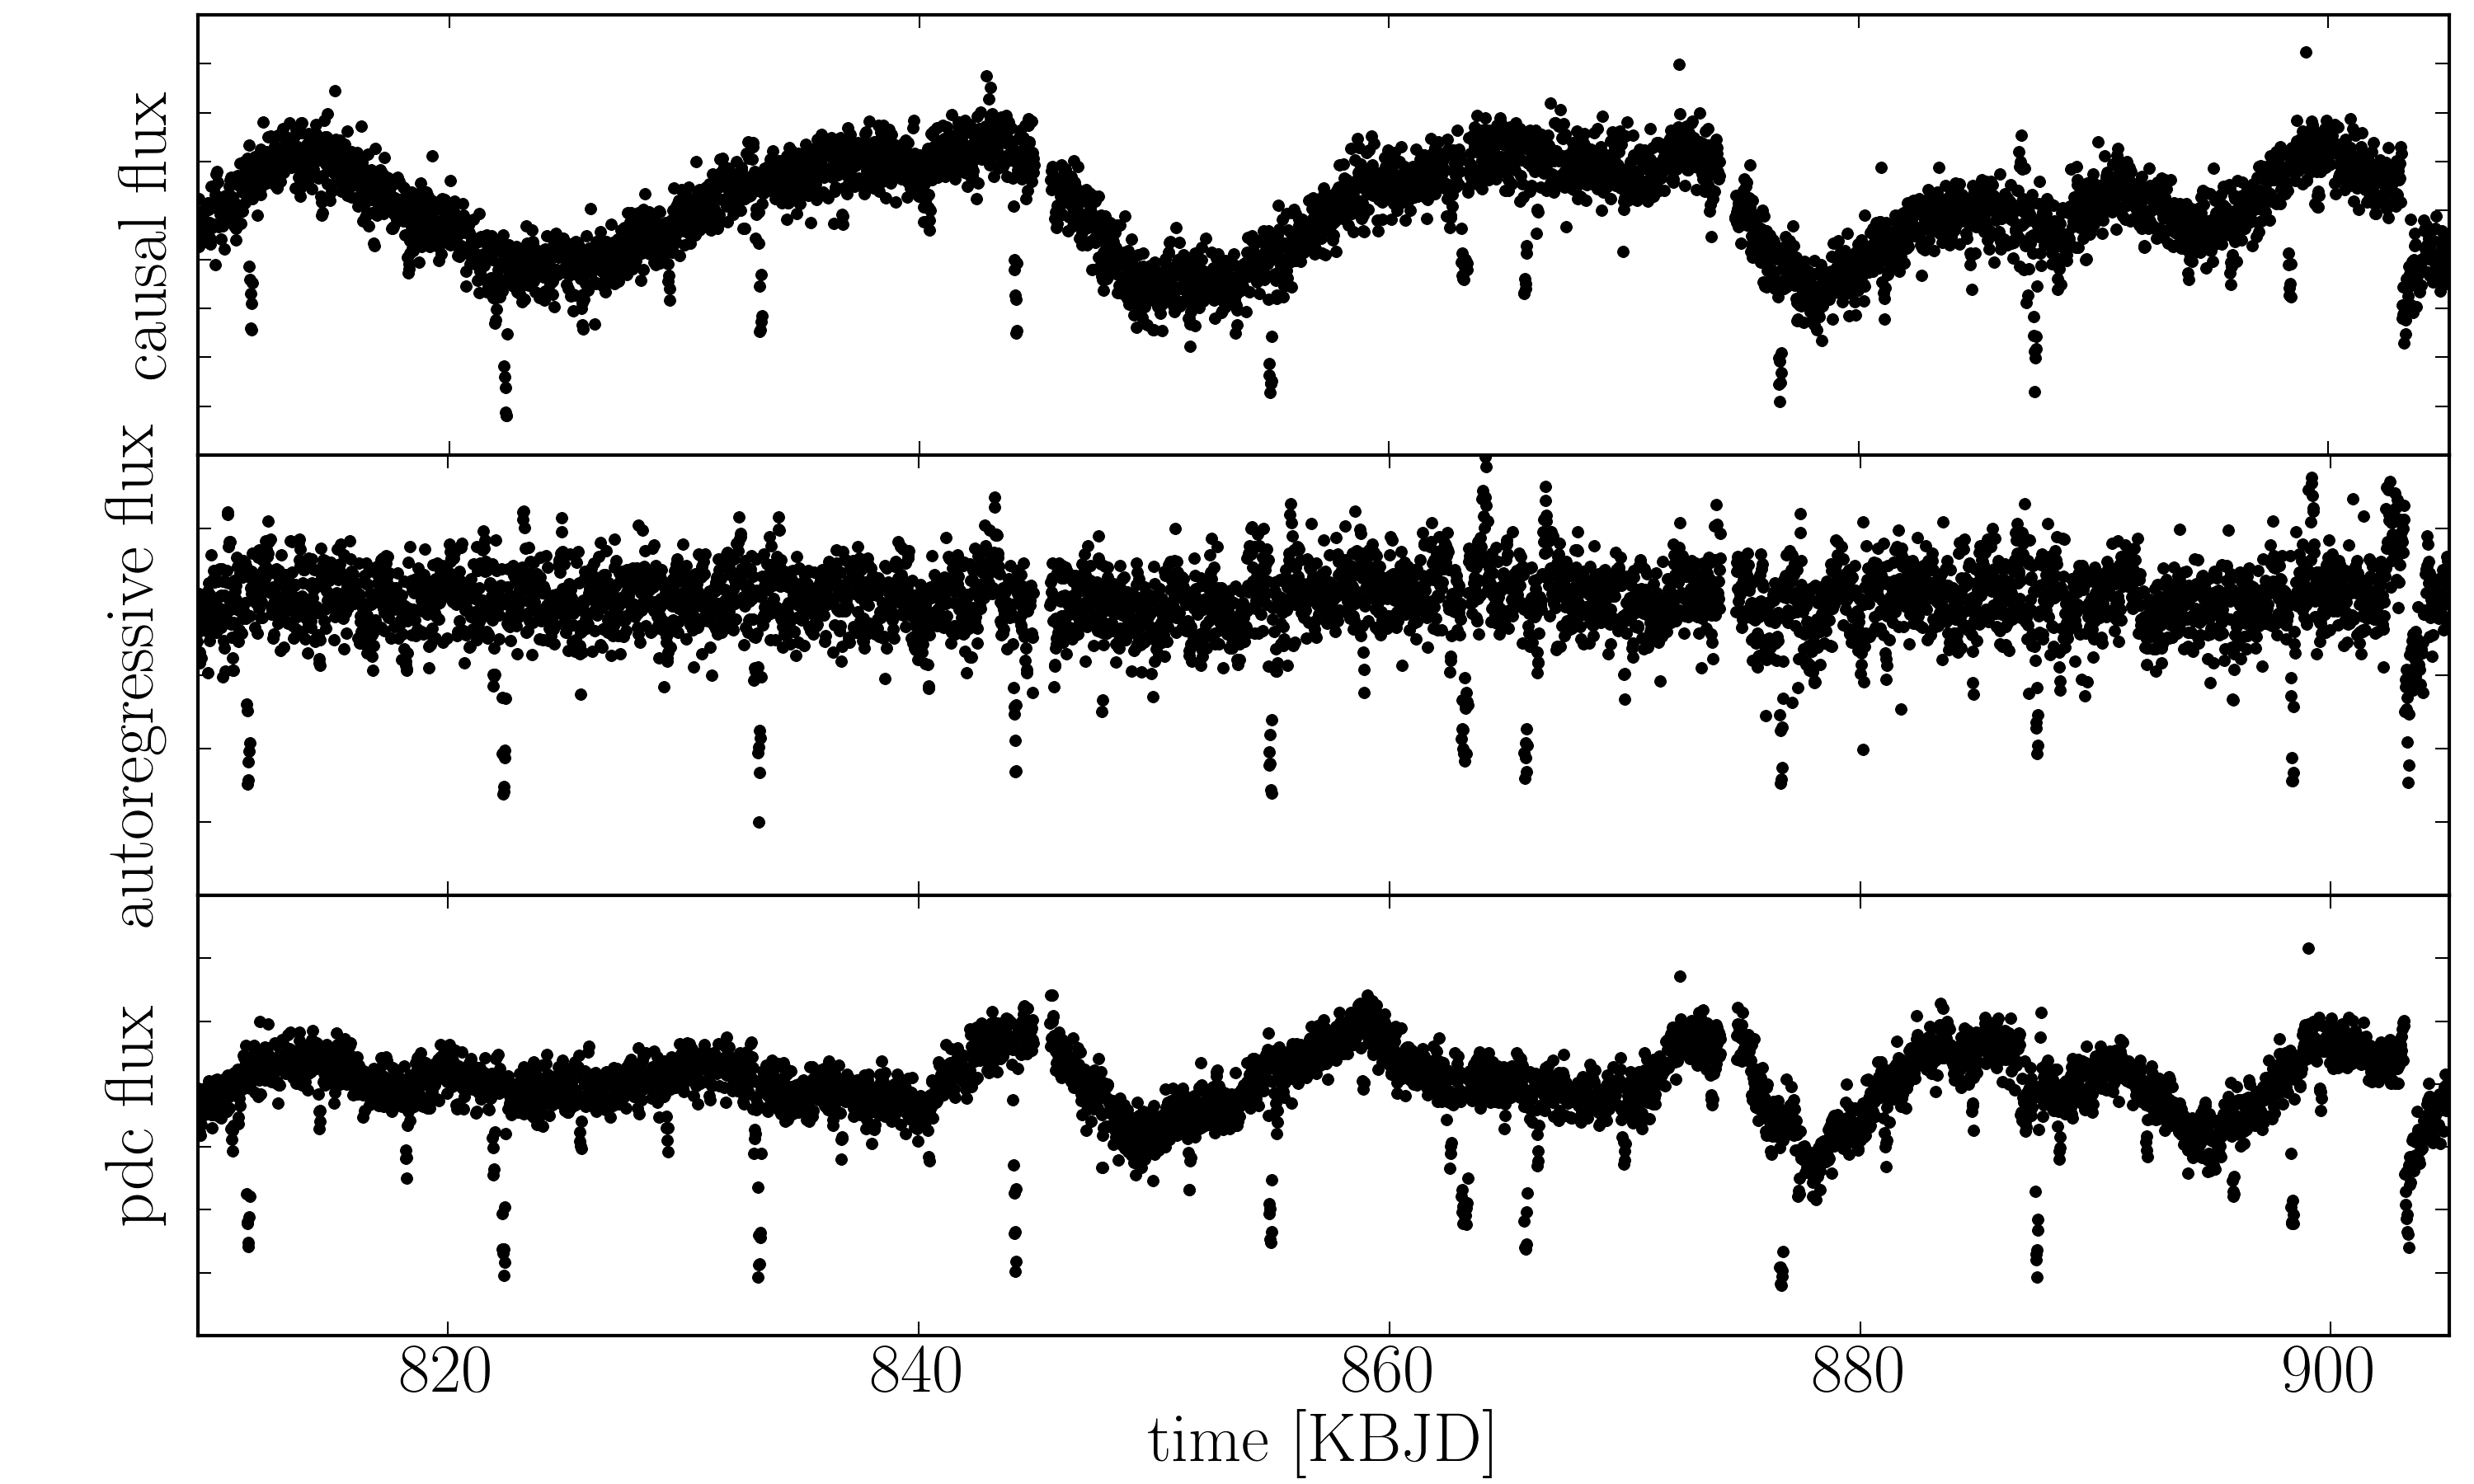
\includegraphics[width=0.9\textwidth]{../whitepaper/kepler-20.png}%
\caption{Results of our data-driven pixel-level systematics model applied to
the quarter 9 observations of \Kepler-20 and compared to the PDC light curve.
\textsl{(top)}~The basic model (equation~\ref{eq:reg-model}) applied to the
pixel time series. This \figurename\ shows the results of coadding the
\emph{residuals} ($f_i (t_k)$ in equation~\ref{eq:reg-model}) using the
optimal aperture from the \Kepler\ pipeline.
\textsl{(middle)}~The same as the top panel using an autoregressive model
(with $\Delta = 12\,\mathrm{hours}$).
\textsl{(bottom)}~The results of doing simple aperture photometry and then
running PDC on the extracted light curve. \label{fig:reg-model}}
\end{figure}

\end{document}
